\documentclass[11pt,aspectratio=169]{beamer}

\usetheme{default}
\usecolortheme{default}
\setbeamertemplate{navigation symbols}{}
\setbeamertemplate{footline}[frame number]
\setbeamercolor{frametitle}{fg=black}
\setbeamerfont{frametitle}{series=\bfseries,size=\large}
\setbeamertemplate{itemize item}{\textbullet}
\setbeamertemplate{itemize subitem}{--}

\usepackage{amsmath,amssymb}

\newcommand{\E}{\mathbb{E}}
\newcommand{\bx}[1]{\textbf{#1}}

% Recurring agenda page; #1 = index of the current section (bolded)
\newcounter{agcur}
\newcommand{\agitem}[2]{\item {\ifnum\value{agcur}=#1\bfseries\fi #2}}
\newcommand{\agenda}[1]{%
  \setcounter{agcur}{#1}%
  \begin{frame}{Agenda}
    \vspace{0.6em}
    \large
    \begin{itemize}\setlength{\itemsep}{11pt}
      \agitem{1}{Review and setup}
      \agitem{2}{Why we cluster}
      \agitem{3}{Common misconceptions}
      \agitem{4}{Recovering the right standard error}
      \agitem{5}{Closing thoughts}
    \end{itemize}
  \end{frame}}

\title{When Should You Adjust Standard Errors for Clustering?}
\author{}
\date{}

\begin{document}

% ---- Title slides ----
\begin{frame}[plain]
  \titlepage
  \subtitle{Abadie, Athey, Imbens, and Wooldridge}
\end{frame}


\begin{frame}[plain]
  \titlepage
\end{frame}

% ======================================================================
\agenda{1}
% ======================================================================

% ---- What are standard errors? ----
\begin{frame}{What are standard errors?}
\begin{itemize}\setlength{\itemsep}{11pt}
  \item Our estimate is one draw from a random process: re-run the study on a fresh sample and you would get a
        slightly different number.
  \item A \bx{standard error} measures how much it moves, i.e., the typical distance between our estimate and the
        truth across hypothetical re-runs.
  \item It is driven by how much \bx{independent information} the sample carries. The basic standard error formula
        assumes every observation is an \bx{independent draw} from the underlying distribution. 
  \item More independent observations $\Rightarrow$ more information $\Rightarrow$ smaller standard error
        (it shrinks at rate $1/\sqrt{n}$).
\end{itemize}
\end{frame}

% ---- What are clustered standard errors? ----
\begin{frame}{What are clustered standard errors?}
\begin{itemize}\setlength{\itemsep}{13pt}
  \item That independence assumption breaks when observations come in \bx{groups} that share common influences (i.e., students in a district,
        workers in a firm).
  \item \bx{Clustered standard errors} relax this assumption by allowing observations to be dependent \emph{within} a group,
        while treating different groups as independent.
  \item Observations carry less information than their count suggests, so your effective
        sample size is closer to the \bx{number of groups} than the number of individuals.
\end{itemize}
\end{frame}

% ---- Anchoring example (moved here; policy bullet removed) ----
\begin{frame}{An anchoring example}
\begin{itemize}\setlength{\itemsep}{8pt}
  \item Suppose we want to estimate the impact of remote learning on student test scores during the pandemic.
  \item \bx{Treatment:} percent of in-person schooling in an academic year
  \item \bx{Outcome:} standardized test scores
\end{itemize}
\vfill
\begin{center}
  \large\bfseries Do we cluster standard errors? By what?
\end{center}
\end{frame}

% ---- Thesis summary (reworked from "the heuristic is wrong") ----
\begin{frame}{The thesis}
Beliefs this paper overturns:
\begin{itemize}\setlength{\itemsep}{4pt}
  \item Clustering matters only if treatment \emph{and} residuals are each correlated
        within clusters.
  \item If clustering changes the standard error, you should do it.
  \item Whether to cluster is a binary choice.
  \item If you add fixed effects, clustering is not needed.
\end{itemize}
\vspace{8pt}
Clustering standard errors is a question about the design:
\begin{itemize}\setlength{\itemsep}{4pt}
  \item How the \bx{sample} was drawn (clustered sampling).
  \item How \bx{treatment} was assigned (clustered assignment).
\end{itemize}
\vfill
\begin{center}
  \itshape Whether to cluster is not something you can determine from the data.
\end{center}
\end{frame}

% ======================================================================
\agenda{2}
% ======================================================================

\begin{frame}{Model-based interpretation}
\begin{itemize}\setlength{\itemsep}{9pt}
  \item \bx{Story:} the textbook motivation: Units in a group share a common unobserved shock, so their
        outcomes are correlated within the group, and clustering accounts for that correlation.
  \item \bx{Problem:} this gives no principled way to choose the grouping. Any within-group correlation would
        justify clustering by that grouping.
    \begin{itemize}\setlength{\itemsep}{3pt}
      \item For example, it could imply you should cluster a clean randomized experiment by gender, even though treatment is assigned independently to each unit.
    \end{itemize}
\end{itemize}
\end{frame}

\begin{frame}{Survey-sampling interpretation}
\begin{itemize}\setlength{\itemsep}{9pt}
  \item \bx{Story:} two-stage sampling --- you first draw a subset of clusters from an infinite 'superpopulation' of
        clusters, then sample units within them. You cluster because of the clusters you \emph{didn't} draw: a
        different draw would have shifted your estimate.
  \item This story is coherent, but it is usually not what researchers actually have in mind --- and it
        rarely fits economics, where we typically observe every cluster in the population.
\end{itemize}
\end{frame}

\begin{frame}{Abadie et al.: the design-based interpretation}
\begin{itemize}\setlength{\itemsep}{11pt}
  \item Clustering is a \bx{design} problem, not a property of the errors. Two independent reasons:
    \begin{enumerate}\setlength{\itemsep}{3pt}
      \item Clustered \bx{sampling} --- which clusters entered the data.
      \item Clustered \bx{assignment} --- how treatment was decided.
    \end{enumerate}
  \item Repeated studies would redraw clusters, or redraw treatment assignments in a way shared within clusters, then uncertainty operates at the cluster level and clustered inference is warranted.
\end{itemize}
\end{frame}

\begin{frame}{Reason 1: clustered sampling}
\begin{itemize}\setlength{\itemsep}{8pt}
  \item You observe a subset of clusters drawn from a larger universe you want to describe. Re-running the study
        would draw \emph{different clusters} --- uncertainty that is correlated within cluster.
  \item Governed entirely by $q$, the fraction of clusters observed:
    \begin{itemize}\setlength{\itemsep}{2pt}
      \item $q=1$: all clusters observed $\Rightarrow$ no sampling reason to cluster (the typical admin-data case).
      \item $q<1$: clusters missing from the target population $\Rightarrow$ cluster.
    \end{itemize}
  \item Whether $q=1$ or $q<1$ depends on the target population and is not visible in the data.
\end{itemize}
\end{frame}

\begin{frame}{Reason 2: clustered assignment}
\begin{itemize}\setlength{\itemsep}{7pt}
  \item Treatment is correlated with the cluster: a program rolled out district by district, local rules,
        policy switches. Two units in the same cluster are more alike in treatment than two in different clusters.
  \item \bx{Model:} each cluster $c$ draws its own treatment probability, with variance $\sigma^2$ \emph{across}
        clusters.
    \begin{itemize}\setlength{\itemsep}{2pt}
      \item $\sigma^2 = 0$: same probability everywhere $\Rightarrow$ random assignment, no reason to cluster.
      \item $\sigma^2$ at its max: whole clusters treated or not $\Rightarrow$ fully clustered (cluster-randomized).
      \item in between: partially clustered.
    \end{itemize}
\end{itemize}
\end{frame}

% ---- Returning to the example: progressive reveal of context ----
\begin{frame}{Returning to our example}
\small
Suppose we want to estimate the impact of remote learning on student test scores during the pandemic.
\begin{itemize}\setlength{\itemsep}{3pt}
  \item \bx{Treatment:} percent of in-person schooling in an academic year
  \item \bx{Outcome:} standardized test scores
\end{itemize}
\vspace{4pt}
\textit{Additional context}
\begin{itemize}\setlength{\itemsep}{3pt}
  \item<2-> Remote-learning policy decisions are made at the district level.
  \item<3-> We have data on a random subset of children from all US schools.
  \item<4-> Wealthier students are significantly more likely to be in districts with in-person schooling.
  \item<5-> When case rates rise above a threshold, a school closes temporarily regardless of district policy.
        Case rates are independent between schools.
  \item<6-> Families can opt out of the district schooling decision by moving their kids to a neighboring school.
\end{itemize}
\end{frame}

% ======================================================================
\agenda{3}
% ======================================================================

% ---- Misconception #1: three slides ----
\begin{frame}{Misconception \#1}
\begin{block}{\normalsize ``Clustering matters only if treatment \emph{and} residuals are each correlated within clusters.''}
\end{block}
\[
  s_i = \tilde W_i\,\hat\varepsilon_i,
  \qquad
  \underbrace{\textstyle\sum_i s_i^2}_{\text{non-clustered}}
  \quad\text{vs.}\quad
  \underbrace{\textstyle\sum_d \Big(\sum_{i\in d} s_i\Big)^2}_{\text{clustered}}
\]
\begin{itemize}\setlength{\itemsep}{9pt}
  \item $s_i$ is unit $i$'s contribution to the estimated effect --- its treatment and its outcome, each after
        partialling out the controls.
  \item \bx{Non-clustered:} square each unit's contribution and add. \bx{Clustered:} sum the contributions
        \emph{within} a district, then square the district total.
  \item So clustering changes the SE exactly when the $s_i$ \bx{line up} (share a sign) within a district.
\end{itemize}
\end{frame}

\begin{frame}{Misconception \#1}
\begin{itemize}\setlength{\itemsep}{11pt}
  \item This needs neither $\tilde W_i$ nor $\hat\varepsilon_i$ to be correlated within district on its own --- it
        needs their \bx{product} to line up.
  \item You can have treatment balanced within every district ($\rho_W \approx 0$) and residuals averaging out
        within every district ($\rho_\varepsilon \approx 0$), and the products $s_i$ can \emph{still} share a sign
        district by district.
  \item Inspecting $\rho_W$ and $\rho_\varepsilon$ separately tells you nothing about whether clustering matters.
\end{itemize}
\end{frame}

\begin{frame}{Misconception \#1 | Example}
\footnotesize
\begin{itemize}\setlength{\itemsep}{3pt}
\item A job-training program is run at 100 sites across the country. We have data from 20 of such sites and would like to estimate the treatment effect on income at all sites. Within each site, applicants are individually randomized into treatment and control. 
\item Because treatment is randomized within each site, treatment status itself is not correlated within a cluster:
$\rho_W \approx 0$.
\item Suppose outcome residuals are uncorrelated within a site because each site has both very high- and low-earning workers:
$\rho_\varepsilon \approx 0$.
\item Suppose sites differ in treatment effects. At strong sites, the treatment effect is much higher than average. At weak sites, the treatment effect is much lower than average.
\item Therefore the coefficient contributions,
\[
s_i = \tilde W_i \hat\varepsilon_i,
\]
line up within site: strong sites push the estimate up, while weak sites push it down.
\item So clustering can matter even when $\rho_W$ and $\rho_\varepsilon$ are near zero. Since the observed sites are only a sample from the target population of sites, clustering by site is warranted.
\end{itemize}
\end{frame}

\begin{frame}{Misconception \#2 | Alter the example}
\begin{block}{\normalsize ``If clustering changes the SE, you should cluster --- and there's no harm if you do.''}
\end{block}

\footnotesize
\setlength{\abovedisplayskip}{2pt}
\setlength{\belowdisplayskip}{2pt}
\begin{itemize}\setlength{\itemsep}{1pt}
\item Alter the previous example: now the target population is exactly the 100 sites, and all 100 sites are represented
in the data.

\item Treatment is still randomized within site, so assignment is not clustered: $\sigma^2=0$.

\item Treatment effects still vary by site:
\[
\tau_c = +1 \text{ in half the sites}, \qquad \tau_c = -1 \text{ in half the sites},
\]
so the finite-population ATE is $0$.

\item The LZ SE is much larger because sites with high effects push the estimate up, and sites with low effects
push it down.

\item But that cross-site variation is not uncertainty from sampling sites: under this design, we did not draw
20 sites from a larger population. We represented all 100.

\item In AAIW's simulation, EHW gives correct coverage, while LZ is far too wide:
\[
\sqrt{V_{\mathrm{EHW}}}=0.007,\quad
\sqrt{V_{\mathrm{LZ}}}=0.051,
\qquad
95% \text{ coverage: } 0.950 \text{ vs. } 1.000.
\]

\item \bx{Takeaway:} a larger clustered SE shows that clustering matters numerically; it does not show that
clustering matches the design.
\end{itemize}
\end{frame}

\begin{frame}{Misconception \#3}
\begin{block}{\normalsize ``The choice is robust \emph{or} clustered.''}
\end{block}

\begin{itemize}\setlength{\itemsep}{9pt}
\item Robust and conventional clustered SEs are two benchmarks, not the only two
logically possible answers.

\item Conventional clustered SEs often go too far: they act as if the observed clusters are a small random sample from a much larger population of clusters.

\item When many or all clusters are observed, and treatment varies within clusters, we can estimate how much of the clustered SE is just cross-cluster treatment-effect heterogeneity rather than true design uncertainty.

\item The correct design-based SE can lie between robust and clustered; AAIW propose corrections that subtract the excess in the conventional clustered variance.
\end{itemize}
\end{frame}

% ======================================================================
\agenda{4}
% ======================================================================

\begin{frame}{Why Liang--Zeger can be too conservative}
The clustered (Liang--Zeger) variance overstates the truth by:
\[
  \mathbb{V}_{\mathrm{LZ}} - \mathbb{V}_{\text{true}}
  = \frac{q}{n}\sum_{c} n_c^2\,\big(\bar\varepsilon_c(1)-\bar\varepsilon_c(0)\big)^2 \;\ge\; 0.
\]
\begin{itemize}\setlength{\itemsep}{7pt}
  \item $\bar\varepsilon_c(1)-\bar\varepsilon_c(0)$: how different cluster $c$'s treatment effect is from the overall treatment effect.
  \item $n_c^2$: squared cluster size. Larger clusters get much more weight.
  \item $q$: the fraction of clusters you observe.
  \item \bx{Takeaway:} LZ treats cross-cluster effect heterogeneity as sampling uncertainty over clusters.
\end{itemize}
\end{frame}

\begin{frame}{Why Liang--Zeger can be too conservative | intuition}
\begin{itemize}\setlength{\itemsep}{10pt}
  \item \bx{Homogeneous effects} $\Rightarrow$ the gap is $0$: clustering is exactly right.
  \item The $n_c^2$ weight makes the over-statement \bx{worst for large clusters} (states, big offices).
  \item The factor $q$ means the excess is \bx{maximal when you observe all clusters} ($q=1$).
  \item This is the formal version of Misconception \#2: The traditional clustering formula treats the spread of cluster-level
        effects as uncertainty in a world where you might have drawn a \emph{different} set of clusters --- but if you saw them all, that is a bad assumption.
\end{itemize}
\end{frame}

\begin{frame}{The fix: estimate the excess and subtract it}
\begin{itemize}\setlength{\itemsep}{8pt}
  \item If treatment varies within clusters, estimate each cluster's own effect ---
        $\hat\tau_c = \bar Y_{c1} - \bar Y_{c0}$ (within-cluster difference in means).
  \item Subtract the size-weighted spread of the $\hat\tau_c$ --- the conservatism LZ built in:
    \[
      \widehat{\mathbb{V}}_{\mathrm{CA}}(\hat\tau)
      = \widehat{\mathbb{V}}_{\mathrm{LZ}}(\hat\tau)
      - \frac{1}{N^2}\sum_{c} N_c^2\,(\hat\tau_c - \hat\tau)^2.
    \]
  \item \bx{Result:} a standard error \emph{between} robust and clustered --- honest about the within-cluster
        dependence that is really there, without the surcharge for clusters you are not missing.
\end{itemize}
\end{frame}

% ======================================================================
\agenda{5}
% ======================================================================

\begin{frame}{Running the decision in practice}
\small
Two substantive questions, asked in order:
\begin{enumerate}\setlength{\itemsep}{3pt}
  \item \bx{Is sampling clustered?} Did you draw a subset of clusters from a larger universe you want to describe?
        (About the target population, not the data. Observe all $\Rightarrow$ no.)
  \item \bx{Is assignment clustered?} Is treatment correlated within cluster --- rolled out by group? (Within-cluster
        variation lets the data inform this.)
\end{enumerate}
\vspace{4pt}
The answers map to actions:
\begin{itemize}\setlength{\itemsep}{2pt}
  \item \bx{Both no} ($q=1,\ \sigma^2=0$): do not cluster --- regardless of whether it changes the SE.
  \item \bx{Assignment clustered} ($\sigma^2>0$): cluster at the assignment level; if all clusters seen with
        within-cluster variation, use $\widehat{\mathbb{V}}_{\mathrm{CA}}$.
  \item \bx{Sampling clustered} ($q<1$) with heterogeneous effects: cluster; LZ is about right.
  \item \bx{Fixed effects:} clustering matters only if treatment effects are heterogeneous.
\end{itemize}
\end{frame}

\begin{frame}{Alternative decision framework}
\textbf{"We leave standard errors as an exercise for the reader"}
    \centering
    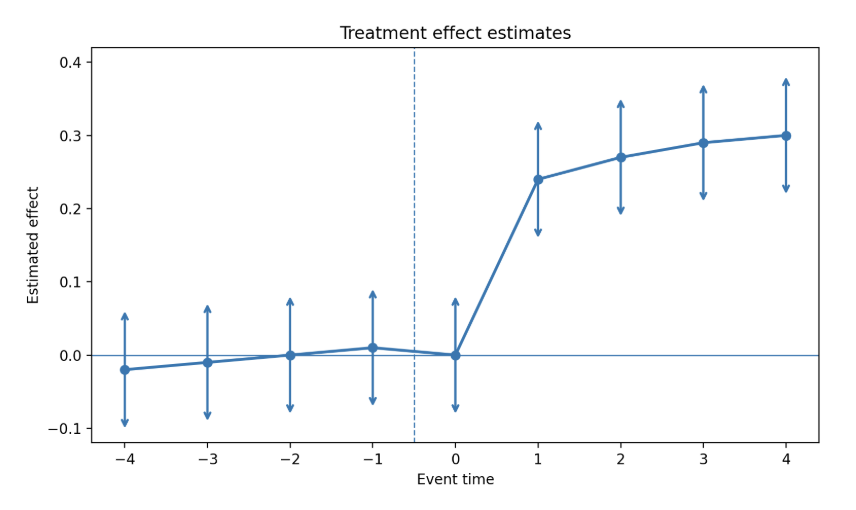
\includegraphics[width=0.8\textwidth]{figures/error_bars.png}
\end{frame}

\end{document}
